% Neural network diagram
% Made with Xematics. Positions are in px (1 px = 0.75 pt), as in the SVG export.
\documentclass[tikz, border=4pt]{standalone}
\definecolor{xm1}{HTML}{FFFFFF}
\definecolor{xm2}{HTML}{FFDDDD}
\definecolor{xm3}{HTML}{CC0000}
\definecolor{xm4}{HTML}{E8F4EA}
\definecolor{xm5}{HTML}{009E73}
\definecolor{xm6}{HTML}{1F2937}
\definecolor{xm7}{HTML}{B8C0CC}
\definecolor{xm8}{HTML}{6B7280}
\begin{document}
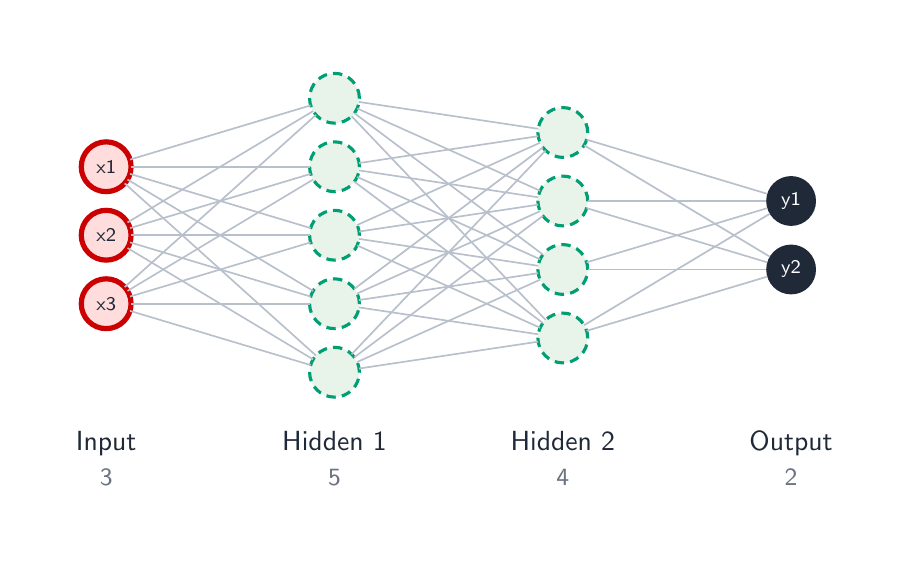
\begin{tikzpicture}[x=0.75pt, y=-0.75pt]
  \tikzset{
    xm input/.style={circle, minimum size=18pt, inner sep=0, outer sep=0, fill=xm2, draw=xm3, line width=1.88pt},
    xm hidden/.style={circle, minimum size=18pt, inner sep=0, outer sep=0, fill=xm4, draw=xm5, line width=1.13pt, dash pattern=on 3.38pt off 2.25pt},
    xm output/.style={circle, minimum size=18pt, inner sep=0, outer sep=0, fill=xm6, draw=none},
    xm edge/.style={draw=xm7, line width=0.6pt},
    xm nodelabel xm6/.style={text=xm6, inner sep=0, font=\sffamily\fontsize{7.5}{9}\selectfont},
    xm nodelabel xm1/.style={text=xm1, inner sep=0, font=\sffamily\fontsize{7.5}{9}\selectfont},
    xm name xm6/.style={text=xm6, inner sep=0, font=\sffamily\fontsize{9.75}{11.7}\selectfont},
    xm size xm8/.style={text=xm8, inner sep=0, font=\sffamily\fontsize{9}{10.8}\selectfont},
  }
  \fill[xm1] (0,0) rectangle (411.07,245.25);
  % Neurons
  \node[xm input] (n-0-0) at (37.82,67) {};
  \node[xm input] (n-0-1) at (37.82,100) {};
  \node[xm input] (n-0-2) at (37.82,133) {};
  \node[xm hidden] (n-1-0) at (147.82,34) {};
  \node[xm hidden] (n-1-1) at (147.82,67) {};
  \node[xm hidden] (n-1-2) at (147.82,100) {};
  \node[xm hidden] (n-1-3) at (147.82,133) {};
  \node[xm hidden] (n-1-4) at (147.82,166) {};
  \node[xm hidden] (n-2-0) at (257.82,50.5) {};
  \node[xm hidden] (n-2-1) at (257.82,83.5) {};
  \node[xm hidden] (n-2-2) at (257.82,116.5) {};
  \node[xm hidden] (n-2-3) at (257.82,149.5) {};
  \node[xm output] (n-3-0) at (367.82,83.5) {};
  \node[xm output] (n-3-1) at (367.82,116.5) {};
  % Connections 0
  \draw[xm edge] (n-0-0) -- (n-1-0);
  \draw[xm edge] (n-0-0) -- (n-1-1);
  \draw[xm edge] (n-0-0) -- (n-1-2);
  \draw[xm edge] (n-0-0) -- (n-1-3);
  \draw[xm edge] (n-0-0) -- (n-1-4);
  \draw[xm edge] (n-0-1) -- (n-1-0);
  \draw[xm edge] (n-0-1) -- (n-1-1);
  \draw[xm edge] (n-0-1) -- (n-1-2);
  \draw[xm edge] (n-0-1) -- (n-1-3);
  \draw[xm edge] (n-0-1) -- (n-1-4);
  \draw[xm edge] (n-0-2) -- (n-1-0);
  \draw[xm edge] (n-0-2) -- (n-1-1);
  \draw[xm edge] (n-0-2) -- (n-1-2);
  \draw[xm edge] (n-0-2) -- (n-1-3);
  \draw[xm edge] (n-0-2) -- (n-1-4);
  % Connections 1
  \draw[xm edge] (n-1-0) -- (n-2-0);
  \draw[xm edge] (n-1-0) -- (n-2-1);
  \draw[xm edge] (n-1-0) -- (n-2-2);
  \draw[xm edge] (n-1-0) -- (n-2-3);
  \draw[xm edge] (n-1-1) -- (n-2-0);
  \draw[xm edge] (n-1-1) -- (n-2-1);
  \draw[xm edge] (n-1-1) -- (n-2-2);
  \draw[xm edge] (n-1-1) -- (n-2-3);
  \draw[xm edge] (n-1-2) -- (n-2-0);
  \draw[xm edge] (n-1-2) -- (n-2-1);
  \draw[xm edge] (n-1-2) -- (n-2-2);
  \draw[xm edge] (n-1-2) -- (n-2-3);
  \draw[xm edge] (n-1-3) -- (n-2-0);
  \draw[xm edge] (n-1-3) -- (n-2-1);
  \draw[xm edge] (n-1-3) -- (n-2-2);
  \draw[xm edge] (n-1-3) -- (n-2-3);
  \draw[xm edge] (n-1-4) -- (n-2-0);
  \draw[xm edge] (n-1-4) -- (n-2-1);
  \draw[xm edge] (n-1-4) -- (n-2-2);
  \draw[xm edge] (n-1-4) -- (n-2-3);
  % Connections 2
  \draw[xm edge] (n-2-0) -- (n-3-0);
  \draw[xm edge] (n-2-0) -- (n-3-1);
  \draw[xm edge] (n-2-1) -- (n-3-0);
  \draw[xm edge] (n-2-1) -- (n-3-1);
  \draw[xm edge] (n-2-2) -- (n-3-0);
  \draw[xm edge] (n-2-2) -- (n-3-1);
  \draw[xm edge] (n-2-3) -- (n-3-0);
  \draw[xm edge] (n-2-3) -- (n-3-1);
  % Labels
  \node[xm nodelabel xm6, anchor=center] at (37.82,67) {x1};
  \node[xm nodelabel xm6, anchor=center] at (37.82,100) {x2};
  \node[xm nodelabel xm6, anchor=center] at (37.82,133) {x3};
  \node[xm nodelabel xm1, anchor=center] at (367.82,83.5) {y1};
  \node[xm nodelabel xm1, anchor=center] at (367.82,116.5) {y2};
  \node[xm name xm6, anchor=base] at (37.82,203.59) {Input};
  \node[xm size xm8, anchor=base] at (37.82,220.35) {3};
  \node[xm name xm6, anchor=base] at (147.82,203.59) {Hidden 1};
  \node[xm size xm8, anchor=base] at (147.82,220.35) {5};
  \node[xm name xm6, anchor=base] at (257.82,203.59) {Hidden 2};
  \node[xm size xm8, anchor=base] at (257.82,220.35) {4};
  \node[xm name xm6, anchor=base] at (367.82,203.59) {Output};
  \node[xm size xm8, anchor=base] at (367.82,220.35) {2};
\end{tikzpicture}
\end{document}
